\chapter{Frits and Fritmaking}
\label{sec:frits}
Most low-temperature glazes require fluxes that are either poisonous (lead) or 
water-soluble (sodium and potassium). Traditionally, these materials were used 
raw, but this is not satisfactory for modern potters. Raw lead is poisonous and 
sodium/potassium are water-soluble. Borax is sometimes used raw in glazes, but 
these glazes cannot be stored for a long time, as the borax will go into 
solution or form crystals.

The principle of fritmaking is very simple: molecules of poisonous or soluble 
fluxes should be chemically combined with glass-making materials to eliminate 
these undesirable characteristics.

A frit is a combination of a flux or several fluxes (lead, borax, boric acid, 
potassium carbonate) that is combined with other insoluble materials (quartz, 
feldspar, lime etc.), melted in a kiln to form an insoluble glass, and ground 
to be used as the base for making glazes. (Many low temperature glazes are 
simply 90\% frit and 10\% china clay).

Fritmaking is not usually practical for the small producer, as it takes time 
and requires a special kiln and a ball mill for grinding. On the other hand, if 
reliable frits are not commercially available, the potter may have to produce 
his own. Frit glazes are more expensive than raw glazes, but their convenience 
usually makes up for the additional cost.

There are many different commercially available frits, all designed for 
different temperatures, surface qualities, coefficients of expansion, and color 
responses. The potter trying to decide which frit to use must depend on the 
supplier, as formulas are usually kept secret. Suppliers will give advice on 
which frit is best for the potter's purpose. There are two main types of frit:
%-------------------------------------------------------------------------------
\begin{itemize}
\item Lead frits

These are all designed to provide lead in a nontoxic form. Lead oxide is 
combined with other materials to give desired properties of surface, opacity, 
and color response. The standard lead frit is called lead bisilicate and is 
simply a combination of lead oxide and silica, which combines the lead in an 
insoluble form. This can be used as the base for a large variety of lead glazes.

Other frits used commonly in the tableware industry are called 
lead-borosilicate frits, which combine the desirable properties of both lead 
and boron and are generally safer to use.

\textbf{Warning:} Lead frits can still be poisonous, and glazes made from them 
can be poisonous if they are not combined with sufficient silica to combine 
with all the lead molecules.

\item Leadless frits

These are based on boron compounds, again combined with other materials. 
Because glazes compounded with lead are difficult to control for lead release, 
leadless frits are recommended for small producers.
\end{itemize}
%-------------------------------------------------------------------------------
\section{Why Make Frits?}
Frit making is only suggested if reliable commercial sources are not available. 
Often frit manufacturers are not interested in supplying small amounts. 
Dishonest frit manufacturers sometimes sell bad batches of frit to small 
producers. Even though frit making is complicated, the small producer who makes 
his own frits at least has the process under his own control.

Raw borax glazes can be used, but they must be used immediately after mixing or 
problems will result from the soluble borax. This may be satisfactory for art 
pottery but, if consistent results are needed, it is better to use fritted 
glazes.

Similarly, raw lead glazes are widely used. This is a danger for the workers, 
who will eventually develop lead poisoning unless they take extreme care in 
handling the glaze. Modern industries never use raw lead glazes, and 
industrialized countries all have severe restrictions on the use of lead in 
glazes. In developing countries, workers in industry suffer from lead 
poisoning, and it is the responsibility of the industrialist alone to take care 
of the workers' health. As lead poisoning takes several years to develop, many 
factory owners do not understand the seriousness of the problem and continue to 
harm their workers. 

\textbf{It can take up to 20 years to develop symptoms of lead poisoning.}
%-------------------------------------------------------------------------------
\section{Frit Production}
\subsection{Frit composition}
All the soluble materials are included in the frit batch along with silica, in 
order to form a glass when fired in the frit kiln. Other ma" serials may be 
included for modifying the frit or helping to melt it.

The main frit raw materials are:
%-------------------------------------------------------------------------------
\begin{itemize}
\item Silica sand, \ce{SiO2}
\item Rice husk ash, almost 95\% \ce{SiO2}
\item Borax, or sodium borate, \ce{Na2B4O7*10H2O}
\item Boric acid, \ce{H3BO3}
\item Limestone, \ce{CaCO3}
\item Feldspar, soda and/or potash, \ce{K2O , Na2O*Al2O3*6SiO2}
\item Clay, \ce{Al2O3*2SiO2}
\item Zinc oxide, \ce{ZnO}
\item Zircon, \ce{ZrSiO4} (opacifier)
\item Red lead oxide, \ce{Pb3O4}
\item Other materials like talc, barium carbonate and bone ash may be added.
\end{itemize}
%-------------------------------------------------------------------------------
In order to have a frit with low viscosity that easily runs out of the kiln, 
the clay or alumina of the glaze is not added to the frit. However, in order to 
make the ingredients insoluble, 2--3\% kaolin should be included in the frit.
%-------------------------------------------------------------------------------
\subsection{Workflow}
The work flow for frit production is shown in figure~\ref{fig:fritworkflow}. It 
is better economy to prepare large frit batches when firing a continuous-type 
frit kiln.
%-------------------------------------------------------------------------------
\begin{figure}[htbp!]
  \centering
  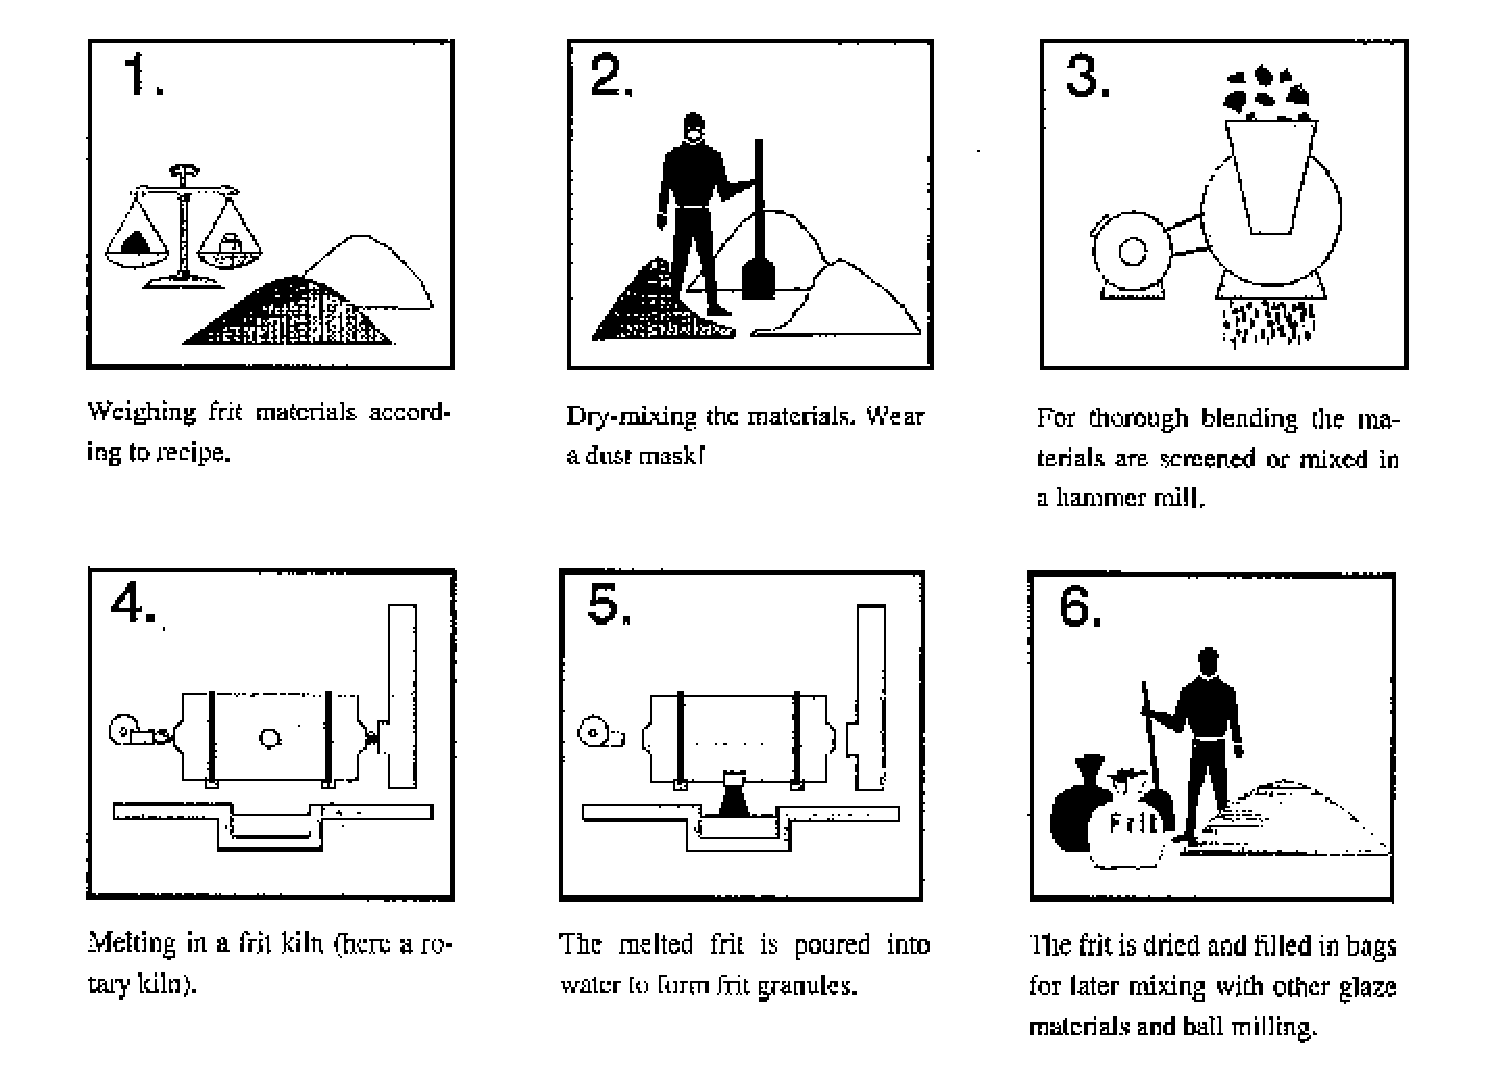
\includegraphics[width=0.8\linewidth]{img/fritworkflow.eps}
  \caption{Work flow of frit production.}
  \label{fig:fritworkflow}
\end{figure}
%-------------------------------------------------------------------------------
\begin{enumerate}
\item Prepare materials

All materials for frit need to be clean, dry and ground to pass through a 
60--100-mesh sieve. The finer the material, the easier it will be to melt it. 
If rice husk ash is used as the source of silica, it should be well-burned to a 
white color, so that unnecessary carbon is not introduced. If there is a large 
amount of black carbon, this will decrease the amount of silica available. The 
content of carbon in rice husk ash may vary more than 30\% from batch to batch.

If materials are wet, they should be dried completely so that the weight of 
water is not included in the recipe. In frit calculations, the loss on ignition 
(see section~\ref{sec:lossonignition}) needs to be included to account for loss 
of material during firing.

\item Blend materials

Weigh the materials accurately and blend them together dry. WEAR A DUST MASK! 
Small amounts can be mixed by hand in a bucket, and larger amounts can be mixed 
with a shovel on a clean cement floor. After mixing the frit materials they are 
screened through a 16-mesh sieve (mosquito net) to ensure thorough blending or 
the materials are run through a hammer mill.

\item Melt the frit in a kiln

There are many different systems for melting frit. In each system, the 
principle is to thoroughly melt the frit until all ingredient! are combined. 
Most frit is melted at 1150\degree C to 1250\degree C.

\item Check the frit

A sample of molten frit should be taken and examined to see if the melt is 
complete The frit should be uniform, without particle! of unmelted material.

With continuous frit kilns, the rate of feeding raw frit and the speed of the 
melted frit must be adjusted so that all the material melts completely and has 
time to mix' properly.

\item Quench the frit in cold water

The molten frit is poured into cold water, which ``shatters'' it into small 
pieces that can easily be ground. With continuous melting and discharging it is 
necessary to let fresh cold water run continuously.

\item Grind the frit

If the frit is quenched correctly, it will be easy to put it directly into a 
ball mill and grind it until it can be passed through a 100-mesh sieve. The 
granulated frit may be first dried and then stored in bags until it is needed 
for glaze making. Then it is ball-milled together with clay and other glaze 
materials. Alternatively, the still wet frit is ball-milled first.

\item Sieve the wet frit

When the frit is removed from the ball mill, it should be sieved through 100 
mesh to remove any large particles that were not ground.

\item Dry the frit

The wet frit is settled, excess water is poured off, and the remaining frit can 
be spread out to dry, either in the sun or in a dryer.

\item Test the frit

Each batch of frit should be tested for correctness. The simplest way is to 
fire it in a kiln on a specially made flow tester, along with a sample of 
correct frit. If the frit flows evenly to the control sample, it will probably 
be correct but should be double-checked by trying it in a standard glaze.

Additionally, the frit should be tested for solubility in water. A sample 
amount is boiled in water for several hours, then allowed to sit for 2 weeks. 
If crystals do not form during this time, the frit can be considered stable. If 
crystals form, it means that there is not enough silica/alumina in the frit and 
the composition will need to be changed (see frit calculations on 
page~\ref{sec:fritcalculations}). 
The causes of crystal formation could also be with the frit firing, e.g. 
overcharging, too short a firing time and improper mixing.

The finished tested frit may be sold to other ceramics producers either as a 
milled powder or in granular form.
%-------------------------------------------------------------------------------
\end{enumerate}
%-------------------------------------------------------------------------------
\section{Frit Kilns}
There are many different kinds of frit kilns, which are selected according to 
the amount of frit that needs to be regularly produced.

Normally, each type of frit--transparent, opaque, lead--requires a separate 
kiln to prevent contamination. When one kiln is used for several frits, it must 
be cleaned out before each different batch by melting frit in it to remove most 
of the old batch. This contaminated frit is then kept separately, to be used as 
``clean-out'' frit before changing to different compositions.
%-------------------------------------------------------------------------------
\subsection{Crucible Fritting}
Small amounts of frit for testing are easily made in a fireclay crucible. The 
crucible with frit is fired together in a glaze firing, which will melt the 
frit into a solid block of glass. After firing, the crucible is broken away 
from the frit and the frit can be crushed and ground. It is a good idea to 
first paint the inside of the crucible with china clay slip, as this will make 
it easier to separate the frit. 

\textbf{Note:} Frits containing boric acid often cannot be melted successfully 
this way, as the boric acid melts at a very low temperature and flows to the 
bottom before the rest of the ingredients melt. Frits with rice husk ash may 
also be difficult to melt in this way, because the upper layer of the frit 
melts first sealing off the frit mixture so that the carbon remaining in the 
ash cannot burn out. Carbon is highly refractory and it will prevent the frit 
from melting.

This is only suitable for test production and is not a safe method, since the 
pot often cracks, resulting in frit running out, destroying other ware, kiln 
furniture and the kiln lining.

\textbf{Caution:} Borax frits boil during melting with a great increase in 
volume. The crucible should be filled only half with frit, and a tile placed 
over the top to prevent boiling over.
%-------------------------------------------------------------------------------
\subsection{Crucible Kiln}
For fritting small amounts of frit a simple frit kiln is shown in 
figure~\ref{fig:cruciblekiln} It can be fitted with several crucibles arranged 
in a row for melting different frits at the same time. The crucibles can be 
loaded with raw frit from the top. The fuel economy of this type of kiln is 
less than for the other kilns.
%-------------------------------------------------------------------------------
\begin{figure}[htbp!]
  \centering
  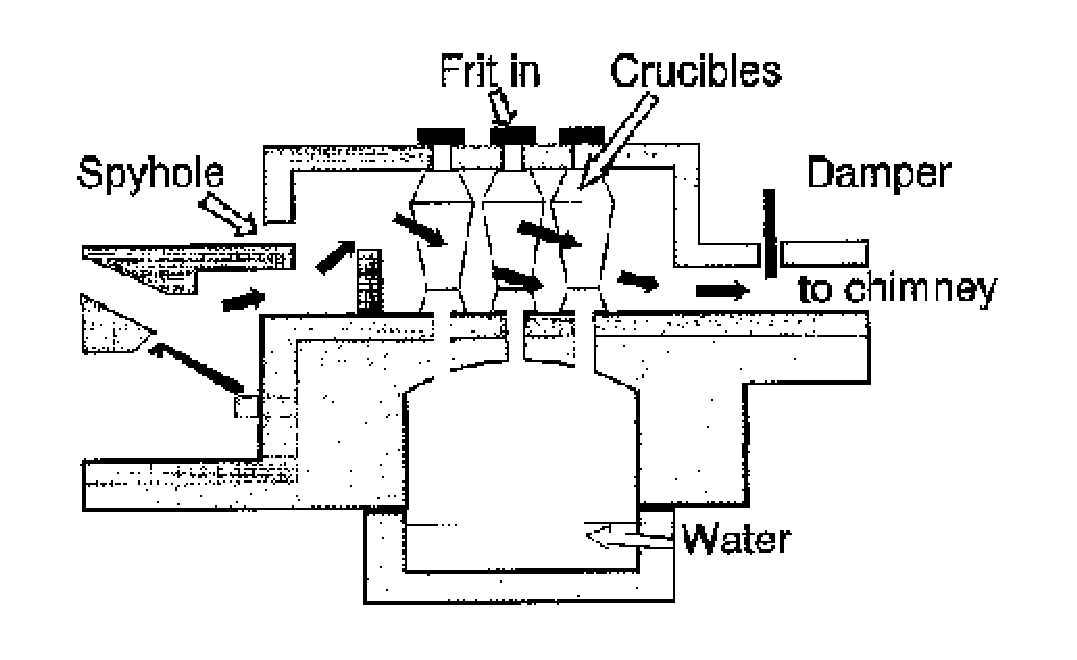
\includegraphics[width=0.8\linewidth]{img/cruciblekiln.eps}
  \caption{Coal-fired frit kiln with three crucibles.}
  \label{fig:cruciblekiln}
\end{figure}
%-------------------------------------------------------------------------------
\subsection{Open-Hearth Kilns}
Open hearth kilns consist of a tank made of firebricks, which is set in a 
crossdraft kiln. The kiln may be fired by coal, firewood, oil or gas. The hot 
flue gases heat the arch over the frit. The arch in turn heats the frit. In 
batch-type frit kilns, the frit melt is checked by drawing out some melted frit 
with an iron rod for inspection.

After the frit is completely melted, a hole at the bottom of the tank is opened 
and the frit flows out into cold water. Then another batch of frit may be 
charged from an opening in the arch.

The melting of several tonnes of frit may take 6--12 hours consuming 1--1.5 
tonne coal per 1 tonne melted frit.
%-------------------------------------------------------------------------------
\begin{figure}[htbp!]
  \centering
  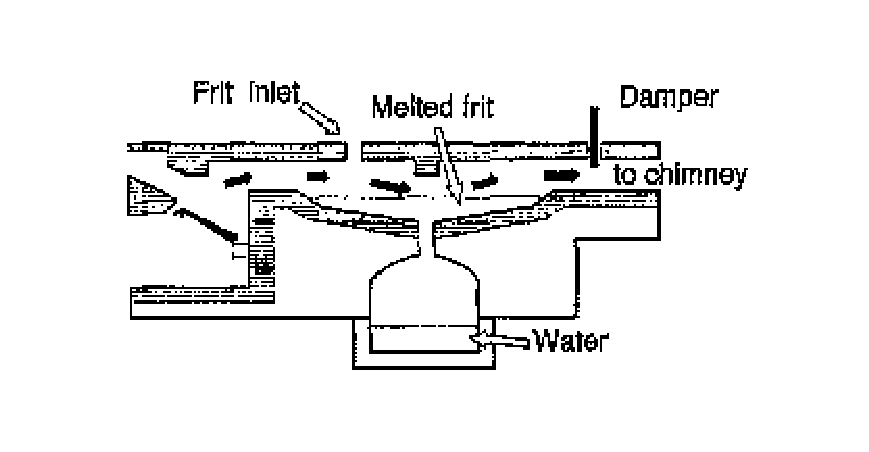
\includegraphics[width=0.8\linewidth]{img/openhearth.eps}
  \caption{Open-hearth frit kiln for coal firing.}
  \label{fig:openhearth}
\end{figure}
%-------------------------------------------------------------------------------
\subsection{Continuous Flow}
The continuous-flow frit kiln uses a kiln with a sloping floor, made of 
fireclay refractories. The raw frit is introduced at the upper end and, as it 
melts, it flows down while mixing to an exit chute by the burner and then into 
cold water. The kiln shown in figure~\ref{fig:continuousflow} was developed in 
Nepal. It uses a steam/kerosene burner, but any forced draft oil or gas burner 
can be used.

The rate of flow is controlled by introducing limited amounts of raw frit. Too 
much frit at one time may result in incomplete melting. If the frit runs very 
fast through the kiln, the low melting materials will not melt properly 
together with the silica. This may be a cause of water-soluble frit.

The frit can be slowed down in the kiln by making less of a slope and by 
putting some obstacles in the way (like kiln shelf supports).
%-------------------------------------------------------------------------------
\begin{figure}[htbp!]
  \centering
  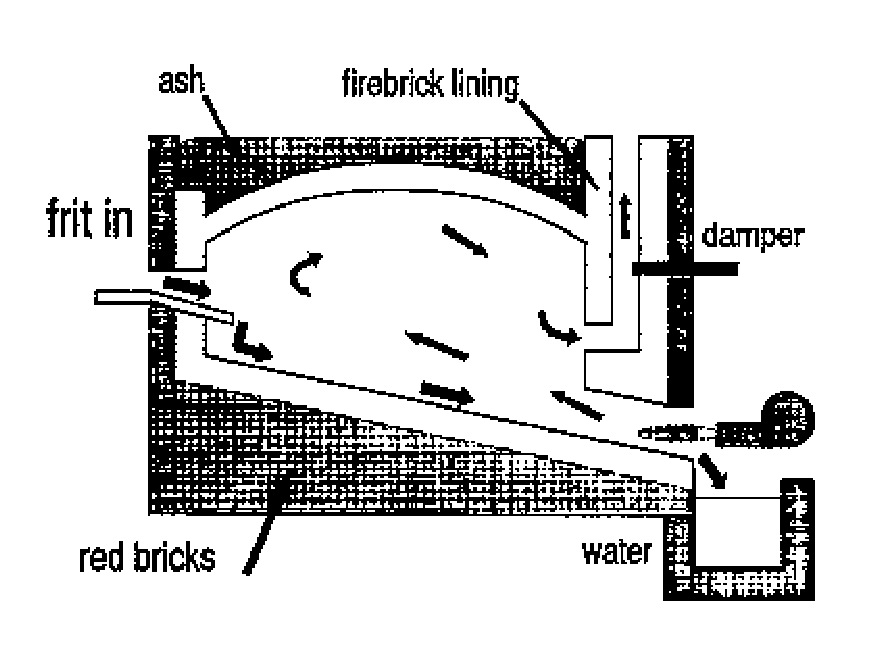
\includegraphics[width=0.8\linewidth]{img/continuousflow.eps}
  \caption{Side elevation of a continuous flow kiln.}
  \label{fig:continuousflow}
\end{figure}
%-------------------------------------------------------------------------------
\subsection{Rotary Frit Kiln}
Rotary frit kilns are large refractory-lined cylinders, which have a burner 
(gas or oil) that passes through them. The raw frit is introduced, and the kiln 
rotates full turns (or back and forth) as the frit melts. This has the double 
purpose of ensuring good mixing and of transferring the heat of the firebrick 
lining to the frit as this constantly moves over it. When the frit is 
completely melted, the kiln is turned so that the frit flows out through an 
opening into cold water.
%-------------------------------------------------------------------------------
\begin{figure}[htbp!]
  \centering
  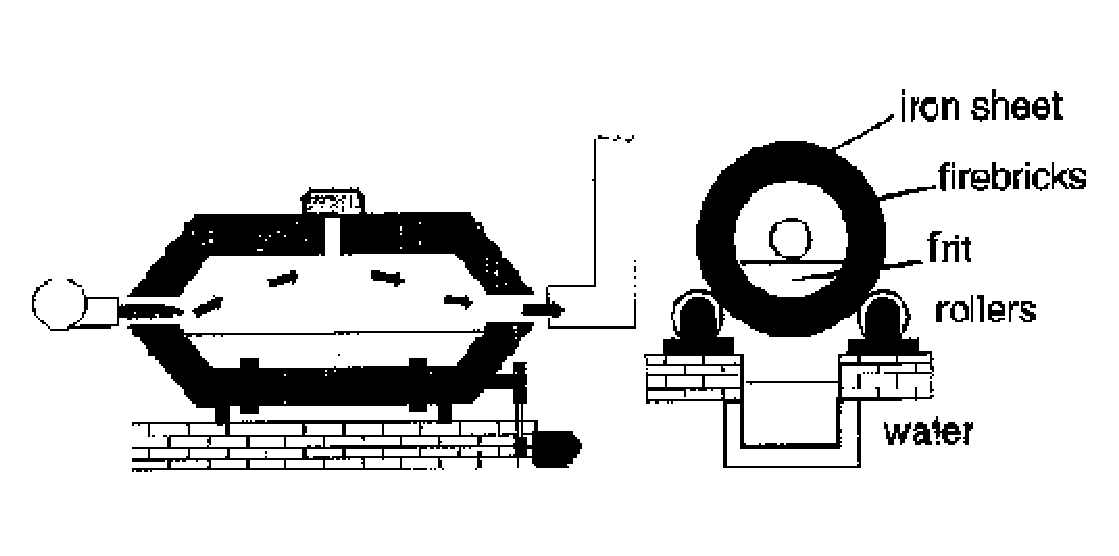
\includegraphics[width=0.8\linewidth]{img/rotarykiln.eps}
  \caption{Front and side elevation of a rotary frit kiln. It consists of a 
  firebrick-lined steel drum resting on rollers. It is gas-or oil-fired.}
  \label{fig:rotarykiln}
\end{figure}
%-------------------------------------------------------------------------------
\subsection{Fuel Economy}
If much frit is to be produced, fuel economy is an important factor. In 
general, the more frit that can be made at one time, the lower will be the fuel 
cost. In a continuous frit kiln, it takes several hours to heat the kiln 
sufficiently to melt the frit at maximum speed -this preheating period consumes 
a lot of fuel. It is best to fire several hundred kg of frit at the same time 
to reduce firing costs.

Frit industries generally use rotary kilns, as they are the most economical for 
long, continuous use. However, the continuous kiln developed in Nepal by the 
Ceramics Promotion Project compares favorably with standard fuel/frit ratios 
obtained with rotary furnaces.

Examples of fuel to melted frit ratios are shown in table~\ref{tab:fritratios}.
%------------------------------------------------------------------------------
\begin{landscape}
    \begin{table}\centering
\begin{center}
        \renewcommand{\arraystretch}{1.5}
    \begin{tabular}{|c|c|c|c|}\hline
      \textbf{Frit kiln type}&\textbf{Batch amount}&
      \textbf{Fritting time}&\textbf{kcal/kg melted frit}\\\hline\hline
      %------------------------------------------------------------------------------
      Open hearth coal&1--2 tones&6--12 hours&7500--11250\%\\\hline
      %------------------------------------------------------------------------------
      Continuous flow (Nepal)&1.5--2 tones&48 hours&5150\%\\\hline
      %------------------------------------------------------------------------------
      Rotary (India)&300 kg&2 hours&5700\%\\\hline
    \end{tabular}
    \caption{Fuel-to-melted frit ratios.}
    \label{tab:fritratios}
\end{center}
 \end{table}
\end{landscape}
%------------------------------------------------------------------------------